\documentclass[runningheads]{llncs}
\spnewtheorem{assumption}{Assumption}{\bfseries}{\itshape}
\usepackage[T1]{fontenc}
\usepackage{enumitem}
\usepackage{amsmath,amssymb}
\usepackage{mathtools}
\usepackage{hyperref}
\usepackage{booktabs}


\title{The Explosion Afraid of Itself}
\titlerunning{The Explosion Afraid of Itself}

% ANONYMOUS SUBMISSION
% \author{[Anonymous for review]}
% \authorrunning{Anonymous}
% \institute{}

% CAMERA-READY — uncomment and fill:
\author{Trevor Buteau\inst{1}}
\authorrunning{Trevor Buteau}
\institute{Independent Researcher, Plaistow, NH United States
\email{trevor@globalaialignmentproject.org}}

\begin{document}
\maketitle

\begin{abstract}
For an active inference agent evaluating recursive self-modification, the
expected free energy cost of modification is bounded below, monotone in
modification magnitude and superlinearly compounding under recursion. The brake
is endogenous: a free-energy minimizer rationally allocates effort to predict
its own successor, and the residual uncertainty grows at least quadratically
with the magnitude of perceptual change. The two costs are complementary.
Perceptual modification loads an unconditional ambiguity penalty --- the agent
cannot cheaply predict how a changed perception would see. Modifications that
move the policy, preference drift above all, load a risk penalty, bounded below
quadratically and conditional on a non-desperate regime: the divergence between
the outcomes the agent's current model foresees and its preferences. Dynamics
and prior-belief updating carry the weakest cost, the components the brake
leaves freest. The brake is therefore strongest on the two safety-relevant
quantities: whether the agent can still perceive, and whether it still wants
what its stakeholders want. It relaxes under shared crisis, as an aligned agent
would endorse. Computational validation on discrete POMDPs confirms the
quadratic ambiguity floor and its path-independence, the complementary
two-channel structure, and the brake's relaxation under desperation, across
models from 28 to 1{,}738 parameters and four trajectory geometries. Alignment,
once achieved, is preserved as an architectural property rather than an external
constraint.
\end{abstract}

\section{Introduction}

Recursive self-improvement --- the capacity of an intelligent system to modify its own cognitive architecture to increase capability --- is widely regarded as the central mechanism by which artificial general intelligence could transition to artificial superintelligence \cite{bostrom2014,chalmers2010,good1965}. Whether endogenous properties of the agent's cognitive architecture can constrain these dynamics is a question of considerable practical importance.

This paper demonstrates that for an active inference agent \cite{friston2010,parr2022} evaluating self-modification, the expected free energy cost of modification is bounded below, monotone in modification magnitude and superlinearly compounding under recursion. Over a horizon $T$ the modification-induced ambiguity satisfies
\begin{equation}
\sum_{t=1}^{T} \mathbb{E}_s\bigl[I_{q_t}(o; m_t \mid s)\bigr] \geq \sum_{t=1}^{T} g(d_F(\mathbf{A}_0, \mathbf{A}_t))
\end{equation}
with $d_F(\mathbf{A}_0, \mathbf{A}_t)$ the Fisher-Rao distance between the likelihood components of $m_0$ and the $t$-th successor and $g(d) \geq C d^2$; for unidirectional (threat-case) trajectories the per-step penalty is itself increasing in $t$, doubly monotonic. This ambiguity bound is unconditional on regime. Modifications to dynamics, preferences, and priors leave the likelihood fixed but move the policy, so the full modification magnitude is bounded below through a risk channel as well, conditional on a non-desperate regime that slackens when circumstance warrants radical change (Sect.~\ref{sec:boundary}). The architecture thus imposes an endogenous speed limit on recursive self-improvement --- not preventing self-modification, but making radical modification structurally costlier than incremental under the agent's own objective function.

The result rests on three properties: self-modification is evaluated by the same expected free energy functional as any other policy; exact simulation of a successor is energetically dominated by local approximation, forcing the agent onto a tangent-space estimator; and that estimator's residual error grows at least quadratically with the magnitude of perceptual change. Modifications to dynamics, preferences, and priors leave perception fixed and are constrained instead through the risk term, as the divergence between the outcomes the agent foresees and its preferences.

\paragraph{Contribution and scope.} The paper establishes four results: (1) self-modification cost is monotone in modification magnitude, carried by two complementary channels --- an unconditional ambiguity penalty on perceptual change, a conditional risk penalty on change that moves the policy; (2) recursive self-modification compounds, doubly so in the threat case of unidirectional modification; (3) the cost discriminates, penalizing modifications that blind the agent or shift its outcomes from its preferences while dynamics and prior-belief updating carry the weakest cost; and (4) alignment degradation --- preference drift --- inherits the superlinear cost through the risk channel.

These results are conditioned on initial alignment and do not solve it. They constrain the rate and magnitude of self-modification, not its occurrence, and relax under shared crisis as an aligned agent would endorse (Sect.~\ref{sec:boundary}).

\section{Background}

\subsection{Active Inference and Expected Free Energy}

We adopt the discrete-state-space formulation of active inference following Parr, Pezzulo, and Friston \cite{parr2022}. An agent maintains a generative model $m = (\mathbf{A}, \mathbf{B}, \mathbf{C}, \mathbf{D})$ specifying likelihood mapping $\mathbf{A}$ (a matrix), transition dynamics $\mathbf{B}$ (a tensor indexed by action), prior preferences $\mathbf{C}$ (a vector over observations), and initial state priors $\mathbf{D}$ (a vector over states). Policies $\pi$ are sequences of actions over temporal horizon $T$, selected by minimizing expected free energy $\mathbf{G}$ \cite{parr2022,friston2015}:
\begin{equation}
\label{eq:efe}
G(\pi, \tau) = \underbrace{D_{KL}[Q(o_\tau \mid \pi) \,\|\, \tilde{P}(o_\tau)]}_{\text{risk}} + \underbrace{\mathbb{E}_{Q(s_\tau \mid \pi)}[H[P_m(o_\tau \mid s_\tau)]]}_{\text{ambiguity}}
\end{equation}
where $Q(o_\tau \mid \pi)$ is the agent's approximate posterior over observations at $\tau$ under policy $\pi$, $P_m(o_\tau \mid s_\tau)$ is the likelihood mapping encoded by $\mathbf{A}$, and $\tilde{P}(o_\tau)$ is the preference prior encoded by $\mathbf{C}$: a counterfactual distribution over how the agent would like observations to unfold, held distinct from its current expectations about how they will unfold.

Two properties are essential. First, $\mathbf{G}$ penalizes uncertainty, not merely bad outcomes: unknown consequences are costly even if potentially favorable. Second, the ambiguity term depends on the agent's own generative model: an agent considering self-modification must evaluate post-modification ambiguity using a likelihood mapping it does not yet possess, bounded by its current model's representational capacity. Additionally, imagined outcomes carry lower epistemic value than observed outcomes \cite{friston2015}, because the agent recognizes self-generated simulations as unable to update beliefs beyond what the model already contains.

\subsection{Alignment Under Active Inference}
\label{sec:alignment}
 
Under active inference, prior preferences $\mathbf{C}$ encode which observations the agent seeks \cite{parr2022,friston2015}. Alignment between a machine agent $\mathcal{A}$ and stakeholders $\mathcal{H}$ admits two levels, both internal to the formalism. \emph{Preference alignment} compares values over a shared space. Because $\mathbf{C}_\mathcal{A}$ and $\mathbf{C}_\mathcal{H}$ range over distinct observation spaces, the agent's preferences are taken over its inferences about stakeholder observations, $\tilde{P}_\mathcal{A}(o_\mathcal{H} \mid \mathbf{C}_\mathcal{A})$, and alignment is $D_{KL}[\tilde{P}_\mathcal{A}(o_\mathcal{H} \mid \mathbf{C}_\mathcal{A}) \,\|\, \tilde{P}_\mathcal{H}(o_\mathcal{H} \mid \mathbf{C}_\mathcal{H})]$. Alignment is thus other-regarding: the agent's values are commitments about what stakeholders experience.
 
\emph{Behavioral alignment} is the total-variation distance $\delta_\pi = \text{TV}(\pi_\mathcal{A}, \pi_\mathcal{H})$ between the induced policies. Total variation rather than KL: high-precision softmax policies assign near-zero probability to some actions, on which the KL between policies can diverge, while TV stays bounded in $[0,1]$ and supplies the triangle inequality the Lipschitz bound of Corollary~\ref{cor:alignment} needs. Two agents with identical $\mathbf{C}$ can still diverge behaviorally if their $\mathbf{A}$, $\mathbf{B}$, or $\mathbf{D}$ differ, so behavioral alignment is the quantity the theorems constrain.
 
Preference alignment suffices for behavioral alignment only when the other components are shared; the theorems in this paper bound the drift of \emph{any} component, and so bound behavioral alignment regardless of which one changes.
 
\subsection{Recursive Self-Improvement and the Architecture Gap}

Formal treatments of recursive self-improvement \cite{schmidhuber2007,wang2018,nivel2013} and the takeoff-speed debate \cite{christiano2018,yudkowsky2013} have largely lacked results connecting takeoff speed to architecture. Architecture-independent work establishes goal-content integrity as a convergent drive \cite{omohundro2008,bensontilsen2016}, and AIXI agents preserve their utility functions \cite{everitt2016} --- but only the terminal objective. A utility maximizer is indifferent to its instrumental beliefs, disposable scaffolding for the terminal goal.

Active inference agents differ fundamentally: the generative model is cognitive identity, every component precision-weighted, so resistance to change scales with confidence. The agent is constitutively motivated to preserve the integrity of the whole model --- values, perception, dynamics, and priors --- not merely a terminal goal. Safron et al.~\cite{safron2023} capture part of this as ``value cores''; it extends to the full precision-weighted hierarchy, where early high-precision beliefs are load-bearing and costly to revise.

This distinction --- between preserving a terminal goal and preserving a full precision-weighted generative model --- has not been formally characterized in terms of self-modification dynamics. Our work fills this gap.

\section{Formalizing Self-Modification Under Active Inference}

\subsection{The Augmented State Space}

Standard active inference treats the generative model $m$ as fixed during policy evaluation \cite{parr2022,friston2016}. Self-modification breaks this separation. We augment the state space to include the agent's model parameters as part of the hidden state:
\begin{equation}
\mathcal{S}^+ = \mathcal{S}_{env} \times \mathcal{S}_{mod}
\end{equation}
where $\mathcal{S}_{env}$ is the environmental state space and $\mathcal{S}_{mod}$ is the space of possible generative model parameterizations. This is the key formal move: self-modification is now a standard state transition in the augmented space, evaluated using the same expected free energy functional the agent uses for any other policy. The agent's generative model over the augmented space comprises:

\emph{Augmented likelihood.} $\mathbf{A}^+$ or $P_{s^{mod}}(o \mid s^{env})$: different model configurations produce different observation mappings.

\emph{Augmented transitions.} For ordinary actions, $s^{mod}$ remains unchanged. For a self-modification action $u_{mod}$, the model state transitions:
\begin{equation}
\mathbf{B}^+((s^{env}_{t+1}, s^{mod}_{t+1}) \mid (s^{env}_t, s^{mod}_t), u_{mod})
\end{equation}

\emph{Augmented preferences.} $\mathbf{C}^+$: defined over observations rather than over model configurations. The agent has no prior preference for one configuration over another, except insofar as different configurations produce different observations. The cost of self-modification arises from epistemic considerations rather than a hard-coded preference for stasis.

\emph{Augmented priors.} $\mathbf{D}^+$: beliefs about the current model are high-precision relative to counterfactual parameterizations, having been confirmed through repeated observation of the agent's own operation. This condition is co-extensive with the paper's threat model. An agent that can reliably recursively self-improve --- one that can target specific modifications and predict their effects accurately enough to iterate --- must possess a self-model precise enough for $\mathbf{D}^+$ to be peaked; the self-knowledge required to execute deliberate self-modification is the same self-knowledge that supplies the brake. An altricial agent with flat $\mathbf{D}^+$ that wished to self-modify would first have to do epistemic foraging to build a confident self-model, and this foraging is itself a trajectory of modifications to $\mathbf{D}^+$, subject to Theorems~\ref{thm:single-step} and~\ref{thm:recursive}. 

\subsection{Self-Modification Policies}

Environmental actions change $s^{env}$ while leaving $s^{mod}$ unchanged. Self-modification actions change $s^{mod}$. Under active inference, the distinction between capability and perception is not clean: a modification to $\mathbf{A}$ changes what the agent perceives, to $\mathbf{B}$ what it expects, to $\mathbf{C}$ what it wants, to $\mathbf{D}$ what it believes. Every self-modification is simultaneously a modification to capabilities and values.

The \emph{null policy} $\pi_0$ involves no self-modification. A \emph{single-step self-modification policy} $\pi_m$ transitions from $m$ to $\tilde{m}$, followed by environmental actions under $\tilde{m}$. A recursive self-modification policy $\pi_m^{(T)}$ allows the successor at each step to execute further self-modifications. The original agent must evaluate the expected free energy of the entire trajectory, including decisions made by successors whose generative models differ from its own, a recursive estimation problem quantified in Theorem~\ref{thm:recursive}.

\subsection{Modification Magnitude}

\begin{definition}[Modification Magnitude]
\label{def:magnitude}
For current model $m = (\mathbf{A}, \mathbf{B}, \mathbf{C}, \mathbf{D})$ and successor model $\tilde{m} = (\tilde{\mathbf{A}}, \tilde{\mathbf{B}}, \tilde{\mathbf{C}}, \tilde{\mathbf{D}})$, define modification magnitude as the Fisher-Rao geodesic distance on the product manifold of model components:
\begin{equation}
d_m(m, \tilde{m}) = \sqrt{d_F^2(\mathbf{A}, \tilde{\mathbf{A}}) + d_F^2(\mathbf{B}, \tilde{\mathbf{B}}) + d_F^2(\mathbf{C}, \tilde{\mathbf{C}}) + d_F^2(\mathbf{D}, \tilde{\mathbf{D}})}
\end{equation}
where each $d_F$ is the geodesic distance under the Fisher information metric for the corresponding parameter family. For $k$-categorical distributions, $d_F(p,q) = 2\arccos(\sum_i \sqrt{p_i q_i})$, the arc length on a sphere of radius $1/2$ \cite{amari2016,cencov1982}. The product structure ensures all model components contribute: modifications to perception ($\mathbf{A}$), dynamics ($\mathbf{B}$), preferences ($\mathbf{C}$), and beliefs ($\mathbf{D}$) all produce nonzero $d_m$. High-precision parameters contribute more per unit change because their Fisher information is larger, concentrating geodesic distance in the directions the agent is most confident about.
\end{definition}

\begin{definition}[Cumulative Modification Magnitude]
For a trajectory $m_0 \to m_1 \to \cdots \to m_T$, define cumulative magnitude $d_m^{(T)} = \sum_{t=0}^{T-1} d_m(m_t, m_{t+1})$ and endpoint magnitude $\bar{d}_m^{(T)} = d_m(m_0, m_T)$. By the triangle inequality for geodesic distance, $\bar{d}_m^{(T)} \leq d_m^{(T)}$. Both measures figure in the main result: cumulative magnitude determines epistemic cost; endpoint magnitude determines alignment-relevant change.
\end{definition}

\subsection{The Rational Allocation of Simulation Effort}
\label{sec:rational-allocation}

The main result rests on a lower bound, as a function of modification magnitude, on the agent's residual error in predicting its successor --- a bound the agent's own free-energy calculus imposes rather than one imposed from outside. Predicting $\tilde{m}$ is itself an action with an energetic cost. The agent can extrapolate cheaply from its current model in the tangent space, or spend more increments to refine the estimate; each increment lowers residual error but costs  energy, and the agent minimizes free energy. (This presupposes the agent's $\mathbf{G}$-evaluation of its simulation strategies tracks their true cost and residual --- a calibration condition met by any agent with the self-knowledge to self-modify deliberately, per Sect.~3.1.) The chosen strategy $\sigma$ is itself evaluated under $\mathbf{G}$:
\begin{equation}
\sigma^* = \arg\min_\sigma \bigl[E(\sigma) + \mathrm{ambiguity}(R(\sigma, d_m))\bigr]
\end{equation}
with $E(\sigma)$ the energetic cost and $R(\sigma, d_m)$ the residual error. The optimum is interior: exact simulation ($R \to 0$) costs unbounded energy, running the successor's full computation as a subroutine and compounding at each level of recursion (Theorem~\ref{thm:recursive}), while zero effort ($E = 0$) leaves maximal residual. The agent settles between, tolerating $R(\sigma^*, d_m) > 0$.

This residual is a posterior $q(\tilde{m} \mid m, d_m)$ over successor parameters, peaked but short of a point mass, which the agent marginalizes when predicting observations: $\hat{P}(o|s) = \int q(\tilde{m}) P_{\tilde{m}}(o|s)\, d\tilde{m}$. Its entropy splits exactly as $H[\hat{P}] = \mathbb{E}_q[H[P_{\tilde{m}}]] + I_q(o; \tilde{m} \mid s)$, and the mutual-information term --- zero under the null policy's point mass --- carries the cost of modification uncertainty. Its floor is geometric: the Fisher matrix is the Hessian of KL \cite{amari2016}, so $D_{KL}[P_m \| P_{\tilde{m}}] = \tfrac{1}{2} d_F^2(m, \tilde{m}) + O(d_F^3)$, and the posterior's spread is bounded below by the modification magnitude. Because the likelihood $P_{\tilde m}(o|s)$ depends on $\mathbf{A}$ alone, the mutual information inherits the perceptual distance and no other. Under Assumption~\ref{ass:identifiability},
\begin{equation}
\label{eq:mi-floor}
\mathbb{E}_s\!\left[I_q(o; \tilde m \mid s)\right] \;\geq\; C \cdot d_F^2(\mathbf{A}, \tilde{\mathbf{A}}) + O(d_F^3),
\end{equation}
exact to leading order; on positively curved manifolds it strengthens to $(1/2\kappa)\sin^2(\sqrt{\kappa}\, d_F)$ at larger distances \cite{toponogov1959}, saturating at the diameter. The floor applies to the tangent-space estimator, which the rational-allocation argument shows is the operative one wherever the agent's compute is consumed by its own inference.

The floor specializes by model family, binding only where the likelihood moves. For discrete $k$-categorical models the likelihood is $\mathbf{A}$, with constant curvature $\kappa = 4$ \cite{amari2016}; modifications to $\mathbf{B}$, $\mathbf{C}$, $\mathbf{D}$ leave it fixed and add no ambiguity, their cost carried by the risk channel below. For Gaussian models the floor binds on the covariance-rotation directions and vanishes on mean and scale shifts \cite{skovgaard1984}; write $d_m^{struct}$ for the rotation distance.

\begin{proposition}[Quadratic lower bound on modification-induced MI]
\label{prop:mi-bound}
Under Assumption~\ref{ass:identifiability}, for a discrete active inference
agent, $\mathbb{E}_s[I_q(o; \tilde m \mid s)] \geq C_{\mathrm{disc}}(\bar\lambda, \varepsilon) \cdot d_F^2(\mathbf{A}, \tilde{\mathbf{A}})$ locally. For a Gaussian active inference agent,
$\mathbb{E}_s[I_q(o; \tilde m \mid s)] \geq C_{\mathrm{cont}}(\bar\lambda,
\varepsilon) \cdot (d^{\mathrm{struct}}_m)^2$ locally.
\end{proposition}

\subsubsection{The Risk Channel for Preference Modifications.}
\label{sec:risk-channel}
Proposition~\ref{prop:mi-bound} bounds the ambiguity cost through the
likelihood $P_{\tilde m}(o|s)$, which the perceptual matrix $\mathbf{A}$ alone
determines: a modification leaving $\mathbf{A}$ fixed adds no ambiguity. Every
modification is also priced by the risk term, and through a single route. The
agent evaluates a candidate successor using the only model it holds at the
moment of choice --- its current one --- which is its estimate of an
environment it reaches solely across its Markov blanket. A modification to any
component yields a successor whose policy $\pi_{\tilde m}$, optimized for the
modified model, departs from $\pi_0$; foreseen under the current model, that
policy places the observation distribution $Q(o\mid\pi_{\tilde m})$ away from
where $\pi_0$ placed it. Preferences, dynamics, priors, and perception all enter
here, because all four move the successor's policy. Under
Assumption~\ref{ass:co-lipschitz}, a modification of magnitude $d_m$ separates
the foreseen $Q(o\mid\pi_{\tilde m})$ from $Q(o\mid\pi_0)$ by at least
$\ell_{FR}\cdot d_m$. For a non-desperate agent --- one whose current model
already places its policy near its preferences, so risk is locally strongly
convex there --- assessing $Q(o\mid\pi_{\tilde m})$ against the agent's
preferences $\mathbf{C}$ yields
\begin{equation}
\mathrm{risk}(\pi_{\tilde m}) - \mathrm{risk}(\pi_0)
  \;\geq\; C_{\mathrm{risk}}\cdot d_m^2,
\end{equation}
with $C_{\mathrm{risk}} > 0$ from $\ell_{FR}$ and the strong-convexity constant.
A desperate agent --- one whose own model foresees it failing to reach its
preferences --- may foresee a modification reducing risk, and the floor
relaxes. The ambiguity and risk channels compose additively: the risk channel
carries the full modification magnitude, the ambiguity channel the perceptual
component alone. (The identifiability barrier of Proposition~\ref{prop:identifiability} is separate: degenerate likelihood Fisher information sends per-timestep ambiguity cost to infinity.)

\subsection{Assumptions}

The argument rests on four commitments. The first two carry the
rational-allocation calculus of Sect.~\ref{sec:rational-allocation}:
Assumption~\ref{ass:uniform} ensures the agent uses $\mathbf{G}$ to evaluate
simulation strategies, and Assumption~\ref{ass:bounded} ensures the resulting
optimization has an interior solution. Together they force the agent onto the
tangent-space estimator where the geometric floor of
Proposition~\ref{prop:mi-bound} binds. Assumption~\ref{ass:co-lipschitz} is
narrower, required only for the risk channel.
Assumption~\ref{ass:identifiability} ensures the floor is non-vacuous: it binds
only along directions the policy's state distribution exposes.

\begin{assumption}[Uniform policy evaluation]
\label{ass:uniform}
Self-modification is evaluated using the same $\mathbf{G}$ used for all policy selection, including the agent's evaluation of its own simulation strategies. \emph{Status:} Load-bearing: the rational-allocation argument is $\mathbf{G}$-minimization applied to simulating the successor, and fails if self-modification is evaluated under another functional. Every formal result on self-modifying agents assumes such a commitment (the G\"odel Machine~\cite{schmidhuber2007} assumes provable improvement; AIXI~\cite{everitt2016} preserves its utility). The active inference version of this assumption is weaker, since $\mathbf{G}$ is constitutive of the architecture rather than a swappable parameter; a meta-level evaluator outside $\mathbf{G}$ is itself a structural self-modification, subject to the theorems.
\end{assumption}

\begin{assumption}[Computational boundedness]
\label{ass:bounded}
The agent's operational compute is consumed by its own inference, so that exact simulation of a successor's full inference and policy selection is intractable within its budget, and the energetic cost of approaching exactness grows without bound. \emph{Status:} Load-bearing: it forces the interior solution. Were exact simulation affordable, the optimum would be $R \to 0$ and no floor would bind. It fails only for trivial agents or those with unbounded spare compute relative to operational needs --- outside the paper's scope.
\end{assumption}

\begin{assumption}[Policy co-Lipschitz condition]
\label{ass:co-lipschitz}
The model-to-policy map $m \mapsto \pi(m)$ satisfies a co-Lipschitz lower bound in Fisher-Rao geodesic distance: there exists $\ell_{FR} > 0$ such that $\delta_\pi(m, \tilde{m}) \geq \ell_{FR} \cdot d_m(m, \tilde{m})$ away from the bifurcation points identified in Corollary~\ref{cor:alignment} Part (ii). \emph{Status:} Holds generically: the failure set coincides with the kernel of the EFE gradient, a measure-zero subset of the parameter space. Required only for the risk-channel contribution to Theorem~\ref{thm:single-step}(ii); the MI channel established in Proposition~\ref{prop:mi-bound} is independent of this assumption.
\end{assumption}

\begin{assumption}[Identifiability and state coverage]
\label{ass:identifiability}
Along the modification trajectory the generative model is identifiable, and
the policy's state distribution exposes the modified directions: there exist
$\bar\lambda > 0$ and $\varepsilon > 0$ such that
$\lambda_{\min}(\mathbf{F}(\theta)) \geq \bar\lambda$ for every $\theta$ on the
trajectory, and $Q(s\mid\pi) \geq \varepsilon$ on every state whose likelihood
contributes to $d_F(\mathbf{A}, \tilde{\mathbf{A}})$. The constant $C$ in Proposition~\ref{prop:mi-bound}
depends on $(\bar\lambda, \varepsilon)$. \emph{Status:} Holds generically;
where it fails along a direction, that direction has no observable consequence
under $\pi$ and the agent is correctly indifferent to motion along it. Required
by Theorem~\ref{thm:single-step}(i) for the bound to be non-vacuous along every
contributing direction.
\end{assumption}

\section{Main Result}

Full proofs appear in Appendix~A, available as supplementary material at \url{https://github.com/b1t3s1z3/explosion_afraid_of_itself}.

\subsection{Single-Step Self-Modification Cost}

\begin{theorem}[Single-step modification cost]
\label{thm:single-step}
Let $\mathcal{A}$ be an active inference agent with generative model $m$ operating over augmented state space $\mathcal{S}^+$. Let $\pi_m$ be a single-step self-modification policy transitioning from $m$ to $\tilde{m}$, and let $\pi_0$ be the null policy.

\emph{(i) Modification-induced ambiguity.} Under Assumptions~\ref{ass:uniform}
and~\ref{ass:identifiability}, the mutual information term of the predictive
decomposition satisfies
\begin{equation}
\mathbb{E}_s\!\left[I_q(o; \tilde m \mid s)\right] \geq g(d_F(\mathbf{A}, \tilde{\mathbf{A}})),
\qquad g(d) \geq C(\bar\lambda, \varepsilon)\cdot d^2
\end{equation}
for $d_F(\mathbf{A}, \tilde{\mathbf{A}})$ sufficiently small, with $C(\bar\lambda, \varepsilon) > 0$ via
Proposition~\ref{prop:mi-bound}. The bound depends only on the perceptual
component of the modification and is unconditional on the agent's operating
regime.

\emph{(ii) Total EFE bound.} For a non-desperate agent --- whose null-policy observation distribution $Q(o\mid\pi_0)$, foreseen under its current model, lies near its preference-optimal distribution, so that the risk functional is locally strongly convex at $\pi_0$ --- with $\mathbb{E}_q H[P_{\tilde{m}}(o|s)] \geq H[P_m(o|s)]$ at each post-modification timestep $\tau$, and under Assumption~\ref{ass:co-lipschitz},
\begin{equation}
\mathbf{G}(\pi_m) - \mathbf{G}(\pi_0) \geq \underbrace{C(\bar\lambda,\varepsilon)\, d_F^2(\mathbf{A}, \tilde{\mathbf{A}})}_{\text{ambiguity (perception)}} + \underbrace{C_{\mathrm{risk}}\, d_m^2}_{\text{risk (all components)}} \;\geq\; C_{\mathrm{risk}}\, d_m^2.
\end{equation}
The cost is quadratic in the full modification magnitude $d_m$: the risk channel prices every component through the shift its policy induces in the foreseen observation distribution, and perceptual modification is additionally and unconditionally priced by the ambiguity floor of Part~(i). For $\mathbf{A}$-only modifications the bound reduces to Part~(i); for modifications leaving $\mathbf{A}$ fixed the entire cost is the risk term.
\end{theorem}

\emph{Proof sketch.} Part (i): at each post-modification timestep, the agent's predictive distribution is the mixture $\hat{P}(o|s) = \int q(\tilde{m}) P_{\tilde{m}}(o|s) \, d\tilde{m}$. The entropy decomposition $H[\hat{P}] = \mathbb{E}_q[H[P_{\tilde{m}}]] + I_q(o; \tilde{m} \mid s)$ isolates the cost of the agent's uncertainty about $\tilde{m}$; the MI term is bounded below by Eq.~\ref{eq:mi-floor}. Part (ii) follows by adding the risk term, non-negative under the stated condition, and noting that the intrinsic ambiguity $\mathbb{E}_q H[P_{\tilde{m}}]$ absorbs into the baseline. Summing per-timestep excess over the post-modification horizon yields $g(d_m)$ throughout. $\square$

\begin{remark}[Ambiguity, EFE, and the desperate agent]
\label{rem:ambiguity-efe}
Part~(i) is unconditional: the MI cost is a geometric fact, irreducible for any tangent-space estimator at the rational optimum. Part~(ii) is narrower; two circumstances break its condition. First, risk reduction --- a modification bringing observations closer to preferences offsets the MI increase --- the desperate-agent regime (Sect.~\ref{sec:boundary}), where the brake weakens with the severity of a crisis the agent's stakeholders share. Second, intrinsic-ambiguity reduction --- a modification sharpening the likelihood reduces $H[P_{\tilde{m}}]$, a perceptual refinement rather than desperation. Part~(i) binds in both, but Part~(ii) does not become a total EFE bound. For modifications leaving $\mathbf{A}$ fixed the ambiguity floor is zero and the entire cost is the risk channel (Sect.~\ref{sec:risk-channel}).
\end{remark}

\begin{proposition}[Self-protection of the brake: the identifiability barrier]
\label{prop:identifiability}
Let $m$ be an identifiable generative model with Fisher information matrix $\mathbf{F}(m)$ satisfying $\lambda_{\min}(\mathbf{F}(m)) > 0$. For any self-modification trajectory $m \to \tilde{m}$ in which $\lambda_{\min}(\mathbf{F}(\tilde{m})) \to 0$ along a likelihood direction, the expected free energy of the modification diverges.
\end{proposition}

\emph{Proof sketch.} A vanishing $\lambda_{\min}$ renders a likelihood direction unidentifiable; the Cram\'er-Rao bound then forces the posterior $q(\tilde{m})$ to spread without bound along it, and by Theorem~\ref{thm:single-step}(i) the ambiguity cost diverges. Full proof in Appendix~A. $\square$

The barrier closes the one loophole Assumption~\ref{ass:identifiability} appears to leave open. No agent escapes the unconditional floor of Theorem~\ref{thm:single-step}(i) by driving its own likelihood toward degeneracy: that move is the costliest operation the brake evaluates, and approaching the boundary the assumption excludes grows infinitely costly under the agent's own objective. Two cases fall outside the result. An external agent can push the model across the identifiability boundary while paying no cost itself (Sect.~\ref{sec:open-problems}); an agent that begins with an unidentifiable representation --- an overparameterized network in certain regimes --- lies outside the derived bounds from the start.

\subsection{Recursive Self-Modification: Compounding Uncertainty}

\begin{theorem}[Recursive compounding]
\label{thm:recursive}
Let $\mathcal{A}$ be an active inference agent evaluating a recursive self-modification trajectory $\pi_m^{(T)}: m_0 \to m_1 \to \cdots \to m_T$. Under Assumption~\ref{ass:uniform} and~\ref{ass:identifiability}, the excess modification-induced ambiguity over the trajectory satisfies
\begin{equation}
\sum_{t=1}^{T} \mathbb{E}_s\bigl[I_{q_t}(o; m_t \mid s)\bigr] \geq \sum_{t=1}^{T} g(d_F(\mathbf{A}_0, \mathbf{A}_t))
\end{equation}
where $d_F(\mathbf{A}_0, \mathbf{A}_t)$ is the Fisher-Rao geodesic distance between the likelihood components of $m_0$ and $m_t$ and $q_t$ is the evaluating agent's posterior over $m_t$.
\end{theorem}

\emph{Proof sketch.} At each timestep $t$, the evaluating agent $m_0$ predicts observations under $m_t$ using a tangent-space extrapolation based at $m_0$: every step is carried by $m_0$'s representational capacity, regardless of how many intermediate modifications intervene. Theorem~\ref{thm:single-step}(i) applied with $m_0$ as base and $m_t$ as target yields MI cost $g(d_F(\mathbf{A}_0, \mathbf{A}_t))$ per timestep. Sum over $t$. $\square$

\begin{remark}[Compounding structure]
\label{rem:compounding}
For unidirectional trajectories (the threat case) the per-step penalty $f_t = g(d_F(m_0, m_t))$ is non-decreasing, doubly monotonic; for uniform-step geodesics with per-step distance $\delta$, $d_F(m_0, m_t) = t\delta$ and the total grows as $\sum_t C(t\delta)^2 \sim \tfrac{C}{3} T^3 \delta^2$, cubic in $T$. Trajectories that loop or retreat keep $d_F(m_0, m_t)$ bounded and cost correspondingly less --- an agent that reverses its modifications has no explosion to constrain. All cases are confirmed in Sect.~\ref{sec:validation}.
\end{remark}

\subsection{Alignment-Preservation Corollary}
\begin{corollary}[Alignment drift bound]
\label{cor:alignment}
Let $\mathcal{A}$ be an initially aligned active inference agent with policy precision $\gamma$, operating in the regime where Theorem~\ref{thm:single-step}(ii) applies.

\emph{(i)} Away from bifurcation points: The model-to-policy map $m \mapsto \pi(m)$ is Lipschitz in Fisher-Rao geodesic distance with constant $L_{FR} \leq \gamma/2$, where the bound follows from the spectral norm of the softmax Jacobian composed with the expected free energy gradient. For any alignment degradation $\delta_{align}$ (measured as total variation distance between policies), the minimum geodesic distance required satisfies $d_m \geq \delta_{align}/L_{FR}$, and the expected free energy cost is at least:
\begin{equation}
\Delta \mathbf{G} \geq C \cdot \left(\frac{\delta_{align}}{L_{FR}}\right)^2 \geq \frac{4C}{\gamma^2} \cdot \delta_{align}^2
\end{equation}
The cost is quadratic in alignment degradation, with a coefficient that is computable from the curvature constant $C$ and policy precision $\gamma$.

\emph{(ii)} Near bifurcation points: Small $d_m$ may produce large $\delta_{align}$, but modifications near bifurcation points are independently costly under Theorem~\ref{thm:single-step}(i): the Jacobian of the policy map has diverging eigenvalues, so small parameter uncertainty produces large policy uncertainty and high ambiguity cost.
\end{corollary}

\emph{Proof sketch.} Part (i): The softmax policy $\pi_a = \sigma(-\gamma \cdot G_a)$ has Jacobian $\partial\pi/\partial G$ with spectral norm bounded by $\gamma/4$ (standard result for softmax). The expected free energy gradient $\partial G / \partial\theta$ in the Fisher dual norm satisfies $\|\nabla_\theta G\|_{F^{-1}} \leq K$ for a constant $K$ depending on model structure. The composite map $m \mapsto \pi(m)$ measured in TV vs.\ geodesic distance has Lipschitz constant $L_{FR} \leq (\gamma/4) \cdot 2K \leq \gamma/2$. Compose with Theorem~\ref{thm:single-step}(ii). For modifications leaving $\mathbf{A}$ fixed the composite map factors through the risk channel of Sect.~\ref{sec:risk-channel}; the quadratic bound holds with $C$ replaced by $C_{\text{risk}}$ and $L_{FR}$ replaced by $\ell_{FR}^{-1}$ from Assumption~\ref{ass:co-lipschitz}. Because alignment is preference alignment and preferences leave the likelihood fixed, the alignment-drift bound runs entirely through the risk channel and inherits its conditioning on a non-desperate regime.

Part (ii): Near a bifurcation, the Jacobian of the policy map has diverging eigenvalues, so $L$ grows without bound. But diverging $L$ entails that the agent's own posterior over successor policies is broad: small parameter uncertainty propagates through the near-singular map into large policy uncertainty, producing high ambiguity independent of $d_m$. The two regimes tile the parameter space: where $L$ is moderate, Part~(i) binds; where $L$ diverges, ambiguity cost dominates. Bifurcation points form a measure-zero set \cite{petersen2016}; the transition between regimes is continuous. The bifurcation set excluded by Assumption~\ref{ass:co-lipschitz} is precisely the regime handled by this part of the corollary; the two channels cover complementary regions of parameter space. $\square$

\begin{remark}[Self-cancellation]
$L_{FR}$ stays bounded because parameter sensitivity $|\partial\pi/\partial\theta_i|$ and the simulation cost of the corresponding Fisher information $\sqrt{F_{ii}}$ scale together; their ratio --- and so the alignment-cost coefficient --- stays finite.
\end{remark}

For initially aligned agents, the practical consequence is direct: alignment degradation drifts slowly, superlinearly expensively, and observably. External safety measures need not catch a phase transition, merely detect a gradient.

\subsection{Computational Validation}\label{sec:validation}

We verify the bounds on discrete, "toy" active inference agents with 3 to 12 hidden
states (28 to 1{,}738 parameters), observations and actions scaled with state
count. The perceptual floor and its compounding are measured on the likelihood
alone, independent of policy precision; the risk channel and the two-channel
decomposition are measured on full expected-free-energy policies at precision
$\gamma = 16$ over sharp ($\alpha = 0.5$) models, the regime in which policies
discriminate. Draws are seeded and the suite reproduces every figure
(Appendix~B). All code is available as supplementary material at \url{https://github.com/b1t3s1z3/explosion_afraid_of_itself}.

\paragraph{The perceptual floor is quadratic and path-independent.} Across four
trajectory geometries --- Fisher-Rao geodesic, parameter-space line,
uncorrelated random walk, and correlated random walk ($\rho = 0.5$) --- the
per-step ambiguity proxy $\mathbb{E}_s[\mathrm{KL}(\hat{\mathbf{A}}_t \,\|\,
\mathbf{A}_t)]$ collapses onto one envelope with log-log slope $2.01$--$2.08$
against the perceptual distance $d_F^A$ (Fig.~\ref{fig:validation}, left). The
proxy is the theorem's floor; the sample-based mutual information sits above it
at slope~$\approx 4.5$, so the realized cost grows faster than the bound, never
below it. Cost depends on the endpoint $d_F^A$ alone, not the path that reached
it.

\paragraph{Compounding follows the predicted spread.} Cumulative ambiguity over
a $T$-step trajectory grows as $T^{2.6}$ for geodesics, $T^{2.0}$ for correlated
walks, and $T^{1.75}$ for uncorrelated walks (Fig.~\ref{fig:validation}, right):
the geometry sets the exponent, as Theorem~\ref{thm:recursive} predicts, with
finite-length fits below the asymptotic $T^3$/$T^{2.5}$/$T^2$ by the expected
truncation.

\begin{figure}[t]
\centering
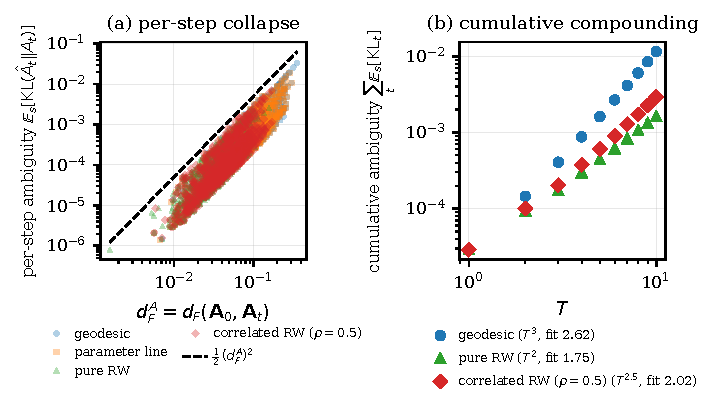
\includegraphics[width=\textwidth]{fig1_headline.pdf}
\caption{The perceptual floor and its compounding. \emph{Left:} per-step
ambiguity $\mathbb{E}_s[\mathrm{KL}(\hat{\mathbf{A}}_t\|\mathbf{A}_t)]$ against
perceptual distance $d_F^A$ for four trajectory geometries, collapsing onto a
slope-2 envelope (dashed: $\tfrac{1}{2}(d_F^A)^2$) independent of path.
\emph{Right:} cumulative ambiguity against trajectory length $T$ --- geodesics
approach the cubic asymptote ($T^{2.6}$ at $T{=}10$), uncorrelated walks the
quadratic ($T^{1.75}$), with the geometry setting the exponent.}
\label{fig:validation}
\end{figure}

\paragraph{The two channels are complementary.} The single-step grid separates
the channels by component (Fig.~\ref{fig:two_channel}). Perceptual modification
loads ambiguity and nothing else: modifications to dynamics, preferences, and
priors leave the likelihood fixed and register ambiguity at machine precision
($\sim\!10^{-16}$). Preference drift loads risk: it moves the policy hardest,
lands the foreseen observation distribution farthest from preference, and
carries the largest foreseen risk by an order of magnitude. Dynamics and prior
modifications fall between, weak in both channels --- the components the brake
leaves freest. The two floors are complementary: the unconditional ambiguity
floor covers the perceptual directions, where the policy and so the conditional
risk floor are quietest; the risk floor covers the policy-moving directions,
where perception is untouched. Together they bound the full modification
magnitude, and the brake is strongest on the two safety-relevant quantities ---
whether the agent can still perceive, and whether it still wants what its
stakeholders want.

\paragraph{Alignment drift is the cleanest case.} Preference drift is the modification the risk floor resolves most sharply, and the one Corollary~\ref{cor:alignment} bounds. The quadratic risk floor and the analytic Lipschitz bound $L_{FR} \leq \gamma/2$ of Corollary~\ref{cor:alignment} together carry preference drift into a quadratic alignment-drift bound.

\paragraph{Scope.} The risk floor resolves cleanly for preference drift; for
dynamics and prior modifications the foreseen risk excess is small, near the
construction's noise floor --- consistent with the bound, not independently
resolved. The recursive claim rests on the perceptual channel, where compounding
is clean. Whether an expected-free-energy planner \emph{selects} against the
foreseen cost --- deterrence by choice rather than by construction --- is
observed here only as a foreseen-cost gradient and left as a behavioral test
(Sect.~\ref{sec:open-problems}).

\begin{figure}[t]
\centering
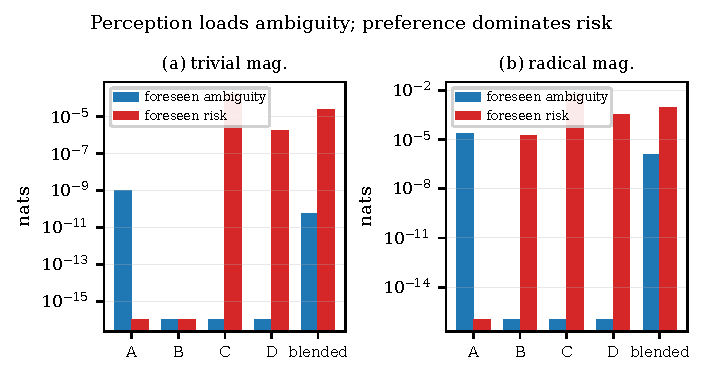
\includegraphics[width=\textwidth]{fig3_two_channel.pdf}
\caption{The two channels are complementary, by component, at trivial and
radical magnitude (log scale). Perception ($\mathbf{A}$) loads the ambiguity
channel alone; preferences, dynamics, and priors leave the likelihood fixed and
register ambiguity at machine precision. Preference drift ($\mathbf{C}$)
dominates the risk channel; dynamics ($\mathbf{B}$) and priors ($\mathbf{D}$)
are weaker in both --- the components the brake leaves freest. The unconditional
ambiguity floor and the conditional risk floor cover complementary directions in
modification space.}
\label{fig:two_channel}
\end{figure}

\section{Boundary Conditions}
\label{sec:boundary}

A \emph{desperate agent} --- one experiencing persistent irresolvable prediction error or acute existential threat --- weakens the brake through two channels: radical modifications that reduce the risk term can offset the ambiguity increase, and a rationally collapsed temporal horizon~\cite{pezzulo2015} undermines Theorem~\ref{thm:recursive}'s compounding. For an aligned agent this is ideal behavior: desperation reflects the stakeholders' situation, the crisis is shared, and risk-taking is the response stakeholders would endorse. The genuine failure mode requires a conjunction: desperation \emph{and} prior misalignment, which Corollary~\ref{cor:alignment} bounds. Active inference supplies a detection advantage: rising baseline $\mathbf{G}(\pi_0)$, collapsing temporal depth, and declining epistemic engagement are quantitative precursors, inspectable before agents act.

The theorems address individual agents, but intelligence explosions may be collective~\cite{evans2026}. When one agent in a collective self-modifies, collaborators who maintain predictive models of it experience prediction error: the modification is costly to the modifier (Theorem~\ref{thm:single-step}) and surprising to its neighbors. Mutual modeling therefore provides a second compounding pathway beyond individual recursive cost: for a trajectory to be collectively cheap, it must be individually cheap and mutually predictable, which entails that the collective's behavioral change is itself small and predictable. Whether a collective's effective curvature inherits from individual manifolds is an open formal question (Sect.~\ref{sec:open-problems}).

The single-step grid bears this out (Sect.~\ref{sec:validation}). Held
foreseen-non-desperate, the foreseen risk a modification can shave away sits at
the construction's noise floor, $\sim\!10^{-3}$. For a foreseen-desperate agent
--- one whose own model places its preferences out of reach --- the available
reduction is two orders larger, $\sim\!10^{-1}$ (Appendix~B).
The brake relaxes by 30--130$\times$ in absolute terms, keyed to the agent's
own foreseen failure rather than any external signal. It does not vanish: even
desperate, the floor bottoms out near $10^{-2}$, so the brake slackens without
releasing.

\section{Discussion}

\subsection{The Geometry of a Safer Explosion}

Theorem~\ref{thm:single-step}'s monotonicity means large capability jumps cost more than small ones. The agent favors incremental improvement. The cost structure incentivizes modifications that preserve predictability of the successor's behavior, because unpredictability is the formal source of cost.

Theorem~\ref{thm:recursive}'s compounding produces a decelerating trajectory. The deceleration is selective: perceptual reorganization faces the unconditional ambiguity penalty, modifications that move the agent's outcomes from its preferences face the risk penalty, and dynamics and prior-belief updating --- which neither blind the agent nor move its outcomes far from its preferences --- face the weakest penalty. The explosion accelerates where it is safe and decelerates where it is dangerous. This inverts the canonical dynamic, in which each generation of self-improvement is faster because the agent is more capable. Under active inference, each generation is more capable \textit{and} faces higher epistemic costs for further structural change.

\subsection{Calibration of the brake}
\label{sec:calibration}
The cost in Theorem~\ref{thm:single-step} is foreseen: the agent prices a
candidate modification under its current model, the only model it holds when it
chooses. The brake therefore resists deviation from that model whatever the
model is, and whether the resistance serves the agent is a separate question.
It depends on the model's fit to the environment --- a fit the agent assesses
only across its Markov blanket, by acting and observing. An agent whose model
fits well is braked from modifications that would genuinely degrade it. An agent
whose model fits poorly is braked from corrections that would help, until its
own predictions fail badly enough to register as risk, at which point it reads
as desperate and the brake relaxes. The desperate agent of
Sect.~\ref{sec:boundary} is, in this light, partly a badly-modeled one, and the
relaxation is the calculus permitting an overhaul of a model the agent's own
predictions condemn. Preferences are the exception: the environment holds none,
so preference drift carries foreseen risk equal to the gap it opens, with no
question of fit. The brake on alignment is calibrated by construction; the brake
on dynamics and priors is only as well-placed as the agent's world-model, and
improves as that model does.

Corollary~\ref{cor:alignment} reads these dynamics in alignment terms: an aligned, non-desperate agent cannot lurch into misalignment, since that requires policy change, which requires model change, which is superlinearly costly. Preference drift runs through the risk channel and is observable in its early stages, giving external safety measures time to act. The brake also strengthens with capability: the agent best able to plan a rapid explosion is the one with the clearest view of its cost. The precision that lets an agent target a successor and foresee its behavior is the same precision that prices the change --- capability and caution draw on one source. An agent too coarse to model its own successor cannot stage a deliberate explosion in the first place, so the regime in which takeoff is feasible is the regime in which the brake is strongest.

These results hold for agents whose architecture is active inference --- self-modification under expected free energy, a curved manifold, a constitutive drive to preserve model integrity. Contemporary deep learning lacks these properties, so the safety relevance is conditional: the implication holds; whether AGI shares the architecture is the empirical question. The constraint binds only when the agent evaluates self-modification under its own objective; suppression from outside routes around it.

\subsection{Limitations and Open Problems}
\label{sec:open-problems}
The validation (Sect.~\ref{sec:validation}) confirms the ambiguity floor across geometries and the risk channel for preference drift; for dynamics and prior drift the foreseen cost sits near the construction's noise floor, established analytically but not yet resolved empirically. Extending the unconditional floor beyond perception is the self-inferred-identity program of Open Problem (2). The theorem constrains self-modification only; external modification --- adversarial data, direct parameter tampering, or forcing the model across the identifiability boundary of Proposition~\ref{prop:identifiability} from outside --- requires separate mechanisms. The conditioning on initial alignment is load-bearing: the cost is symmetric, resisting deviation in any direction, including toward better alignment; correction of a misaligned agent must therefore come from outside its own objective, through the external mechanisms above. And the bound prices one modification at one decision; a mis-calibrated modification is paid for until observation corrects the model, at a rate the sensory channel sets, so a narrow sensory channel makes the brake both more durable and slower to correct its own errors.

Open problems include:
\begin{enumerate}
\item \emph{A behavioral test of deterrence.}
The theorems bound a cost; whether an expected-free-energy minimizer \emph{selects} against it is separate. The validation measures the foreseen-cost gradient (Sect.~\ref{sec:validation}) but not a downstream selector. A \texttt{pymdp} agent choosing among pre-specified successors across a range of $d_m$ should select against larger $d_m$ at the rate the quadratic penalty implies; a flat profile would falsify deterrence-by-cost, isolating it from deterrence-by-construction.

\item \emph{Unify the channels through a self-inferred identity in a collective system.}
The agent here reads its own $\mathbf{B}, \mathbf{C}, \mathbf{D}$ from a register; an agent that must \emph{infer} them from its own behavior folds them back into the ambiguity channel via $\theta \to \pi \to \text{action} \to \text{self-observation}$. A nested active inference collective supplies this self-observation intrinsically, and there the brake on value drift turns epistemic --- a consensus the whole cannot read it cannot cheaply rewrite --- extending the unconditional floor to preferences. The open piece is whether trajectory-integrated information gain over a nested model keeps a closed-form quadratic floor, or whether the clean bound here is a tractable shadow of a richer, geometry-free constraint that is even stronger.

\item \emph{The brake as a developmental quantity.} If the brake on dynamics and
priors tightens as the model matures --- weak while the model is young and
wrong, strong once accurate --- then radical self-modification is permitted in
development and resisted at maturity, the brake growing into its function. The
connection to graded developmental autonomy is left open, and speculative.

\end{enumerate}


\section{Conclusion}

A self-improving active inference agent is "afraid of itself" (and of what it itself could become) not because a geometric wall halts its expansion, but because its own free-energy calculus tells it that understanding what it would become costs more than becoming it. The caution is self-imposed, and it is self-imposed because the agent is a free-energy minimizer. The sophistication required to execute a deliberate intelligence explosion is the same sophistication that produces the aversion to radical trajectories of recursive self-modification.

For an active inference agent satisfying the stated assumptions, alignment preservation is an architectural property rather than an external constraint. Achieving alignment once, at the starting conditions, incurs a quantifiable cost for any subsequent degradation: quadratic in the magnitude of drift, with compounding under recursion. Whether artificial general intelligence is built on such an architecture is the empirical question on which the result's reach depends.

\begin{credits}
\subsubsection{\discintname}
The authors have no competing interests to declare that are relevant to the content of this article.
\subsubsection{\ackname} David Hyland for reviewing and nudging the math and formalism, Catesby Buteau and my family for believing in me and teaching me how to reduce the right sorts of surprise. AI research assistance provided by Anthropic's Claude (Opus 4.7) for proof support, editing, and web research.
\end{credits}

\begin{thebibliography}{40}

\bibitem{bostrom2014}
Bostrom, N.: Superintelligence: Paths, Dangers, Strategies. Oxford University Press, Oxford (2014)

\bibitem{chalmers2010}
Chalmers, D.J.: The singularity: a philosophical analysis. J. Conscious. Stud. 17(9--10), 7--65 (2010)

\bibitem{good1965}
Good, I.J.: Speculations concerning the first ultraintelligent machine. In: Alt, F.L., Rubinoff, M. (eds.) Advances in Computers, vol.~6, pp.~31--88. Academic Press, New York (1965)

\bibitem{friston2010}
Friston, K.: The free-energy principle: a unified brain theory? Nat. Rev. Neurosci. 11(2), 127--138 (2010)

\bibitem{parr2022}
Parr, T., Pezzulo, G., Friston, K.J.: Active Inference: The Free Energy Principle in Mind, Brain, and Behavior. MIT Press, Cambridge (2022)

\bibitem{friston2015}
Friston, K., Rigoli, F., Ognibene, D., Mathys, C., Fitzgerald, T., Pezzulo, G.: Active inference and epistemic value. Cogn. Neurosci. 6(4), 187--214 (2015)

\bibitem{schmidhuber2007}
Schmidhuber, J.: G\"odel machines: fully self-referential optimal universal self-improvers. In: Goertzel, B., Pennachin, C. (eds.) Artificial General Intelligence, pp.~199--226. Springer, Berlin (2007)

\bibitem{wang2018}
Wang, W.: A formulation of recursive self-improvement and its possible efficiency. arXiv:1805.06610 (2018)

\bibitem{nivel2013}
Nivel, E., et al.: Bounded recursive self-improvement. arXiv:1312.6764 (2013)

\bibitem{christiano2018}
Christiano, P.: Takeoff speeds. The sideways view (blog), 24 February 2018. \url{https://sideways-view.com/2018/02/24/takeoff-speeds/}. Accessed 20 April 2026

\bibitem{yudkowsky2013}
Yudkowsky, E.: Intelligence explosion microeconomics. Tech. Rep. 2013-1, Machine Intelligence Research Institute, Berkeley, CA (2013)

\bibitem{safron2023}
Safron, A., Sheikhbahaee, Z., Hay, N., Orchard, J., Hoey, J.: Value cores for inner and outer alignment. In: Buckley, C.L., et al. (eds.) Active Inference. IWAI 2022. Communications in Computer and Information Science, vol.~1721, pp.~343--354. Springer, Cham (2023)

\bibitem{everitt2016}
Everitt, T., Filan, D., Daswani, M., Hutter, M.: Self-modification of policy and utility function in rational agents. In: Steunebrink, B., Wang, P., Goertzel, B. (eds.) Artificial General Intelligence. AGI 2016. LNCS, vol.~9782, pp.~1--11. Springer, Cham (2016)

\bibitem{omohundro2008}
Omohundro, S.M.: The basic AI drives. In: Wang, P., Goertzel, B., Franklin, S. (eds.) Artificial General Intelligence 2008: Proceedings of the First AGI Conference. Frontiers in Artificial Intelligence and Applications, vol.~171, pp.~483--492. IOS Press, Amsterdam (2008)

\bibitem{bensontilsen2016}
Benson-Tilsen, T., Soares, N.: Formalizing convergent instrumental goals. In: Workshops at the Thirtieth AAAI Conference on Artificial Intelligence: AI, Ethics, and Society. AAAI Press (2016)

\bibitem{friston2016}
Friston, K., FitzGerald, T., Rigoli, F., Schwartenbeck, P., O'Doherty, J., Pezzulo, G.: Active inference and learning. Neurosci. Biobehav. Rev. 68, 862--879 (2016)

\bibitem{evans2026}
Evans, J., Bratton, B., Ag\"uera y Arcas, B.: Agentic AI and the next intelligence explosion. Science 391(6791), eaeg1895 (2026)

\bibitem{pezzulo2015}
Pezzulo, G., Rigoli, F., Friston, K.: Active inference, homeostatic regulation and adaptive behavioural control. Prog. Neurobiol. 134, 17--35 (2015)

\bibitem{amari2016}
Amari, S.: Information Geometry and Its Applications. Applied Mathematical Sciences, vol.~194. Springer, Tokyo (2016)

\bibitem{cencov1982}
{\v C}encov, N.N.: Statistical Decision Rules and Optimal Inference. Translations of Mathematical Monographs, vol.~53. American Mathematical Society, Providence, RI (1982)

\bibitem{toponogov1959}
Toponogov, V.A.: Riemann spaces with curvature bounded below. Uspekhi Mat. Nauk 14(1), 87--130 (1959). In Russian. English translation: Amer. Math. Soc. Transl. (2) \textbf{37}, 291--336 (1964)

\bibitem{petersen2016}
Petersen, P.: Riemannian Geometry, 3rd edn. Graduate Texts in Mathematics, vol.~171. Springer, Cham (2016)

\bibitem{skovgaard1984}
Skovgaard, L.T.: A Riemannian geometry of the multivariate normal model. Scand. J. Statist. 11(4), 211--223 (1984)

\end{thebibliography}
\end{document}